% =====================================================================
% Corridor environment parameterization (Option B framing)
% REPLACES the earlier "microsimulation calibrated to GEH<5 (FHWA)" wording.
% Paste into methods.tex (the SO1.1 / calibration subsection) via Overleaf.
% Cite keys used already exist in thesis_refs.bib: Wangsun, Rodriguez2023Cooperative.
% Add Figures/calibration_validation.png to the repo Figures/ folder.
% =====================================================================

\subsection{Corridor Environment Parameterization}
\label{subsec:corridor-parameterization}
The study corridor is represented in SUMO as the ordered sequence of the
direction-code-6 stops of Route~801, with inter-stop travel and stop dwell
\emph{parameterized directly from the CapMetro APC record} rather than
reconstructed from a street-level road-network microsimulation. This
empirical-parameterization approach follows the abstract-corridor modeling that
is standard in the bus-holding reinforcement-learning literature, in which the
control problem is driven by realistic travel-time, dwell, and demand
distributions rather than by full traffic microsimulation
\cite{Wangsun,Rodriguez2023Cooperative}.

For each inter-stop segment, the free-flow running time is set to the empirical
median of $\mathrm{rev\_seconds}-\mathrm{dwell\_time}$---the open-to-open time
net of the originating stop's dwell, which avoids double-counting that dwell;
each stop's dwell is set to its empirical median $\mathrm{dwell\_time}$; and
passenger demand at each stop is drawn from the mean boardings observed in the
APC data (Section~\ref{subsec:data-processing}). All values derive from the
229{,}421-event direction-code-6 subset.

To confirm that the SUMO environment reproduces the empirical corridor behavior
from which it is parameterized, simulated segment running times were compared
against their APC targets over the reduced study corridor
(Table~\ref{tab:corridor-validation}, Figure~\ref{fig:corridor-validation}).
Every segment satisfies $\mathrm{GEH}<5$---well within the $>\!85\%$ acceptance
threshold adopted for the environment---with an overall RMSPE of $8.2\%$; the
residual is attributable to vehicle acceleration and deceleration at stops.
Street-level microsimulation of the corridor road network from OpenStreetMap is
identified as future work.

% ---------------------------------------------------------------------
\begin{table}[htbp]
\centering
\caption{Corridor environment validation: simulated (SUMO) versus empirical
(APC) segment running times over the reduced study corridor.}
\label{tab:corridor-validation}
\begin{tabular}{lrrrr}
\toprule
Segment & Observed (s) & Simulated (s) & GEH & \% err \\
\midrule
5857--5858 & 156 & 166 & 0.83 & $+6.8$ \\
5858--4540 & 119 & 129 & 0.90 & $+8.4$ \\
4540--467  & 163 & 176 & 1.00 & $+8.0$ \\
467--5859  & 106 & 117 & 1.04 & $+10.4$ \\
5859--5606 & 193 & 207 & 0.99 & $+7.3$ \\
\midrule
\multicolumn{5}{l}{\small All segments GEH $<5$; RMSPE $=8.2\%$.} \\
\bottomrule
\end{tabular}
\end{table}

\begin{figure}[htbp]
\centering
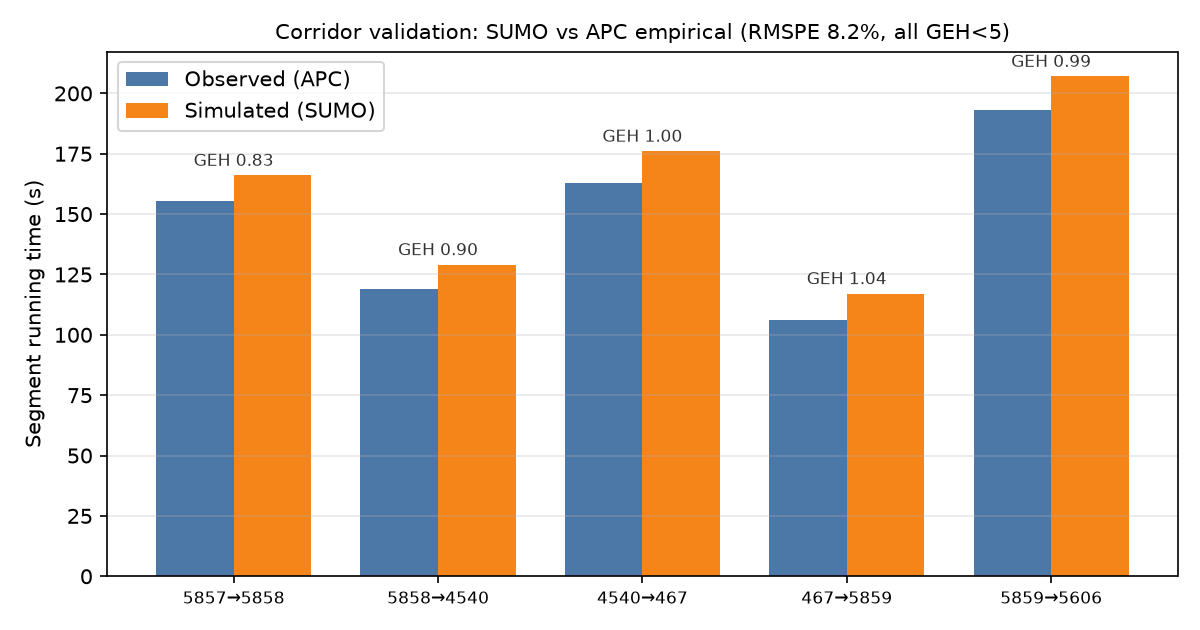
\includegraphics[width=0.8\textwidth]{Figures/calibration_validation.png}
\caption{Simulated (SUMO) versus empirical (APC) segment running times over the
reduced study corridor; every segment satisfies GEH $<5$ (RMSPE $8.2\%$). The
small positive bias reflects bus acceleration/deceleration at stops.}
\label{fig:corridor-validation}
\end{figure}
